% Adjust these for the path of the theme and its graphics, relative to this file
%\usepackage{beamerthemeFalmouthGamesAcademy}
\usepackage{../../beamerthemeFalmouthGamesAcademy}
\usepackage{multimedia}
\graphicspath{ {../../} }

% Default language for code listings
\lstset{language=C++,
        morekeywords={each,in,nullptr}
}

\input{../listings_GLSL}
\newcommand{\fullbleed}[1]{
\begin{frame}[plain]
	\begin{tikzpicture}[remember picture, overlay]
		\node[at=(current page.center)] {
			\includegraphics[width=\paperwidth]{#1}
		};
	\end{tikzpicture}
\end{frame}
}

\newcommand{\picturepage}[2]{
\begin{frame}[plain]
	\begin{tikzpicture}[remember picture, overlay]
		\node[at=(current page.center)] {
			\includegraphics[width=\paperwidth]{#1}
		};
		\draw<1>[draw=none, fill=black, opacity=0.9] (-1,-5.2) rectangle (current page.south east);
		\node[draw=none,text width=0.96\paperwidth, align=right] at (5.5,-5.5) {\tiny{#2}};
	\end{tikzpicture}
\end{frame}
}

\newcommand{\notepicx}[5]{
\begin{frame}[plain]
	\begin{tikzpicture}[remember picture, overlay]
		\node[at=(current page.center)] {
			\includegraphics[width=\paperwidth]{#1}
		};
		\node[draw=none, fill=black, text width=#5\paperwidth] at ([xshift=#3, yshift=#4] current page.center) {\small{#2}};
	\end{tikzpicture}
\end{frame}
}

\newcommand{\notepic}[4]{
	\notepicx{#1}{#2}{#3}{#4}{0.4}
}

% For strikethrough effect
\usepackage[normalem]{ulem}
\usepackage{wasysym}

\usepackage{pdfpages}

% http://www.texample.net/tikz/examples/state-machine/
\usetikzlibrary{arrows,automata}

\newcommand{\modulecode}{COMP260}\newcommand{\moduletitle}{Distributed Systems}\newcommand{\sessionnumber}{5}

\begin{document}
\title{\sessionnumber: Textures and models}
\subtitle{\modulecode: \moduletitle}

\frame{\titlepage} 

\begin{frame}
	\frametitle{Learning outcomes}
	\begin{itemize}
		\item \textbf{Explain} how a complex 3D model is represented in memory
		\item \textbf{Explain} how a 2D texture image can be wrapped onto a 3D model
		\item \textbf{Write} programs which draw textured meshes to the screen
	\end{itemize}
\end{frame}

\part{Basic texture mapping}
\frame{\partpage}

\begin{frame}{Loading textures from a file}
	\begin{itemize}
		\item The \textbf{SDL\_Image library} lets us load images from JPG, PNG, BMP etc.
		\pause\item Steps:
			\begin{itemize}
				\pause\item Load the image with \lstinline{IMG_Load}
				\pause\item Create a texture with \lstinline{glGenTextures}
				\pause\item Bind the texture with \lstinline{glBindTexture}
				\pause\item Load the pixel data into the new texture with \lstinline{glTexImage2D}
				\pause\item Set the texture filtering modes with \lstinline{glTexParameteri} (more on this later)
			\end{itemize}
	\end{itemize}
\end{frame}

\begin{frame}{Texture coordinates}
	\begin{itemize}
		\item We use \textbf{UV coordinates} to refer to points in a texture
		\pause\item $u$ axis is horizontal and ranges from 0 (left) to 1 (right)
		\pause\item $v$ axis is vertical and ranges from 0 (bottom) to 1 (top)
		\pause\item (So really just another name for $xy$ coordinates in texture space)
		\pause\item Basic idea of texture mapping: give each vertex a $uv$ coordinate, and interpolate across the triangle
	\end{itemize}
\end{frame}

\begin{frame}{UV coordinates}
	\begin{center}
		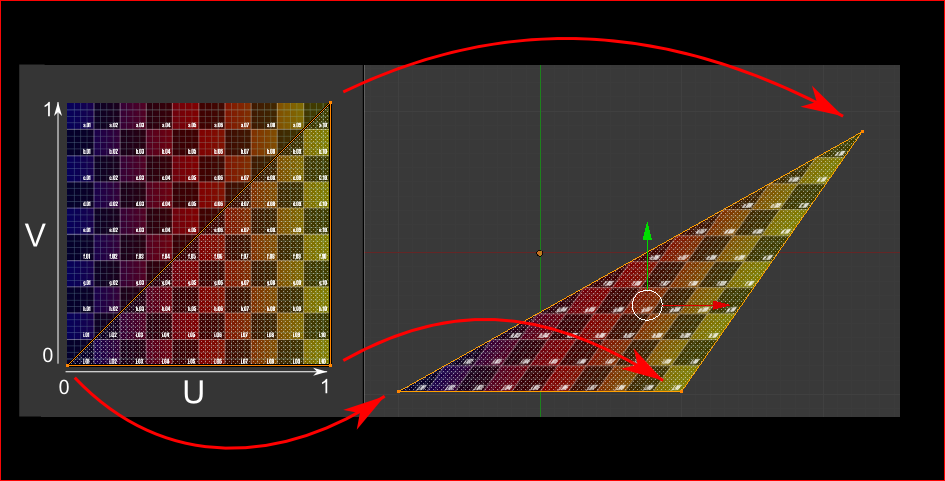
\includegraphics[width=\textwidth]{uv}
	\end{center}
\end{frame}

\fullbleed{character_texture}

\begin{frame}[fragile]{Textures in GLSL}
	Fragment shader:
	
	\begin{lstlisting}[language=GLSL]
in vec2 textureCoords;
uniform sampler2D textureSampler;

void main()
{
    fragmentColour = texture(textureSampler, textureCoords);
}
	\end{lstlisting}
\end{frame}

\begin{frame}[fragile]{Texture filtering}
	\pause
	\begin{lstlisting}
glTexParameteri(GL_TEXTURE_2D, GL_TEXTURE_MIN_FILTER, GL_LINEAR);
glTexParameteri(GL_TEXTURE_2D, GL_TEXTURE_MAG_FILTER, GL_LINEAR);
	\end{lstlisting}
	\begin{itemize}
		\item \textbf{Linear interpolation} (\lstinline{GL_LINEAR})
			smooths between pixels
		\pause\item \textbf{Nearest neighbour} (\lstinline{GL_NEAREST})
			is pixelated but may be slightly faster
		\pause\item \textbf{Anisotropic filtering} improves the quality of linear interpolation
			but is slower
		\pause\item \textbf{Mip-mapping} pre-calculates scaled down versions of the texture ---
			improves quality but costs memory
	\end{itemize}
\end{frame}

\begin{frame}{Texture dimensions}
	\begin{itemize}
		\item In the old days, OpenGL required textures to have \textbf{power of two} dimensions
			\begin{itemize}
				\pause\item $2, 4, 8, 16, 32, 64, 128, 256, 512, 1024, \dots$
			\end{itemize}
		\pause\item Nowadays \textbf{non-power of two (NPOT)} textures are widely supported
		\pause\item Still better to stick to powers of two as some things work better (e.g.\ mipmapping)
		\pause\item NB: \textbf{rectangular} textures are fine, but \textbf{square} textures make UV coordinates saner
	\end{itemize}
\end{frame}

\begin{frame}
	\begin{center}
		Texture Mapping Example
	\end{center}
\end{frame}


\part{Transparency}
\frame{\partpage}

\begin{frame}{Alpha}
	\begin{itemize}
		\pause\item We are used to working with colours in \textbf{RGB} space
		\pause\item We can also work in \textbf{RGBA} space, where A = alpha = transparency
		\pause\item $A=0 \implies$ fully transparent
		\pause\item $A=1$ (or $A=255$) $\implies$ fully opaque
	\end{itemize}
	\pause
	\begin{center}
		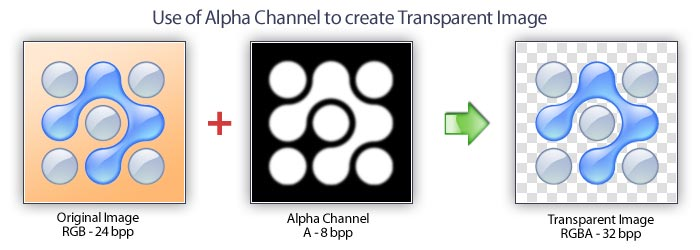
\includegraphics[width=\textwidth]{alpha_channel}
	\end{center}
\end{frame}

\begin{frame}[fragile]{Alpha in OpenGL}
	\begin{itemize}
		\pause\item Use \lstinline[language=GLSL]{vec4} instead of \lstinline[language=GLSL]{vec3} for colours
		\pause\item Textures can have an \textbf{alpha channel}
			\begin{itemize}
				\pause\item PNG supports alpha channels, JPG and BMP do not
			\end{itemize}
		\pause\item Need to enable \textbf{alpha blending}
	\end{itemize}
	\pause
	\begin{lstlisting}
glEnable(GL_BLEND);
glBlendFunc(GL_SRC_ALPHA, GL_ONE_MINUS_SRC_ALPHA);
	\end{lstlisting}
	\begin{itemize}	
		\pause\item Other values can be passed to \lstinline{glBlendFunc} for special effects
			(e.g.\ \textbf{additive blending} is often used for particle effects simulating
				light, fire, explosions etc.)
	\end{itemize}
\end{frame}

\begin{frame}{Transparency and depth testing}
	\begin{itemize}
		\pause\item Recall we are using \textbf{depth testing}
			\begin{itemize}
				\pause\item Each fragment on screen remembers its \textbf{depth} (distance from the camera)
				\pause\item A new fragment is drawn \textbf{only if} its depth value is \textbf{less} than the current depth value
				\pause\item I.e.\ don't draw objects that should be behind something that was already drawn
			\end{itemize}
		\pause\item But if the object in front is (semi-)transparent, we want to see the object behind it!
		\pause\item Solution: draw semi-transparent objects \textbf{after} opaque objects,
			and in \textbf{back to front} order
		\pause\item Further discussion: {\footnotesize\url{http://www.opengl-tutorial.org/intermediate-tutorials/tutorial-10-transparency/}}
	\end{itemize}
\end{frame}


\part{More meshes}
\frame{\partpage}

\begin{frame}{SOH CAH TOA}
	\begin{center}
		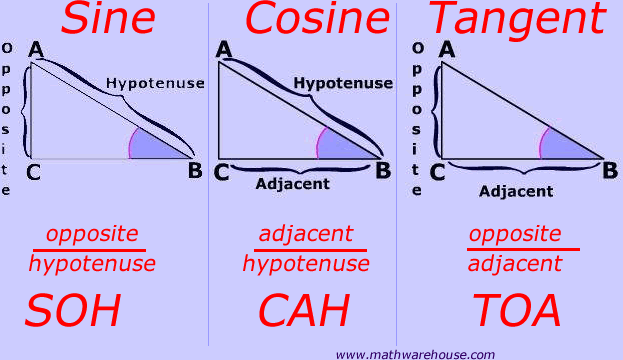
\includegraphics[width=\textwidth]{sohcahtoa}
	\end{center}
\end{frame}

\begin{frame}{Drawing a circle}
	\begin{columns}
		\begin{column}{0.48\textwidth}
			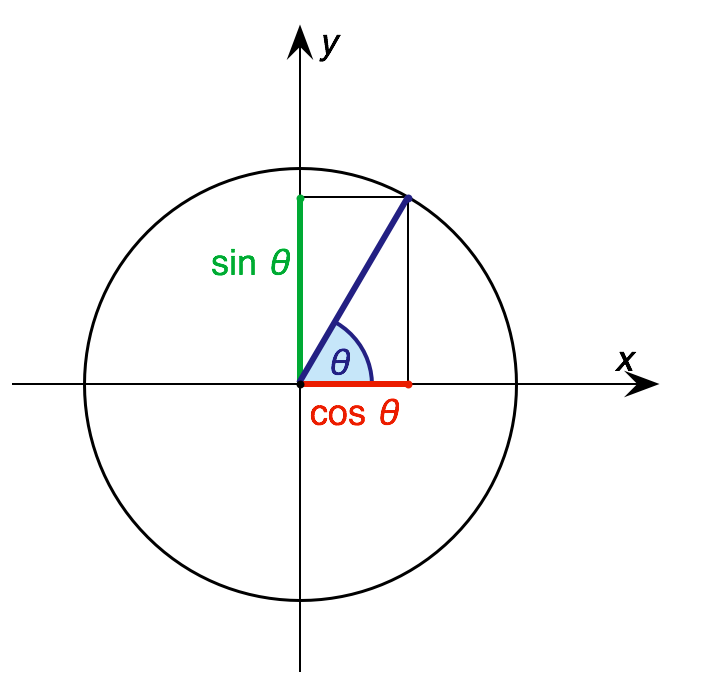
\includegraphics[width=\textwidth]{unit_circle}
		\end{column}
		\begin{column}{0.48\textwidth}
			\pause Circle of \textbf{radius} $r$
			
			\pause $\therefore$ hypotenuse = $r$
			
			\vspace{2ex}
			
			\pause $\cos \theta = \frac{\text{adjacent}}{\text{hypotenuse}} = \frac{x}{r}$
			
			\pause $\therefore x = r \cos \theta$
			
			\vspace{2ex}
			
			\pause $\sin \theta = \frac{\text{opposite}}{\text{hypotenuse}} = \frac{y}{r}$
			
			\pause $\therefore y = r \sin \theta$

			\vspace{2ex}
			
			\pause NB: this works even if $\cos \theta$ and/or $\sin \theta$ are negative
				(i.e.\ if $\theta$ is not between $0^\circ$ and $90^\circ$)
		\end{column}
	\end{columns}
\end{frame}

\begin{frame}{Drawing a cylinder}
	\begin{center}
		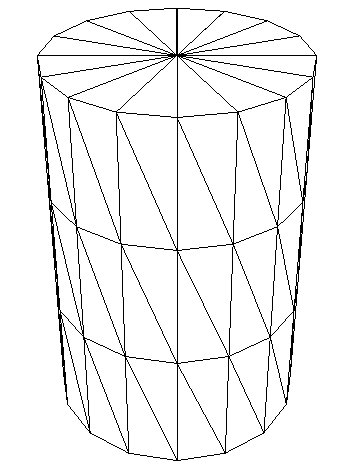
\includegraphics[height=0.8\textheight]{cylinder}
	\end{center}
\end{frame}

\begin{frame}{Drawing a sphere}
	\begin{center}
		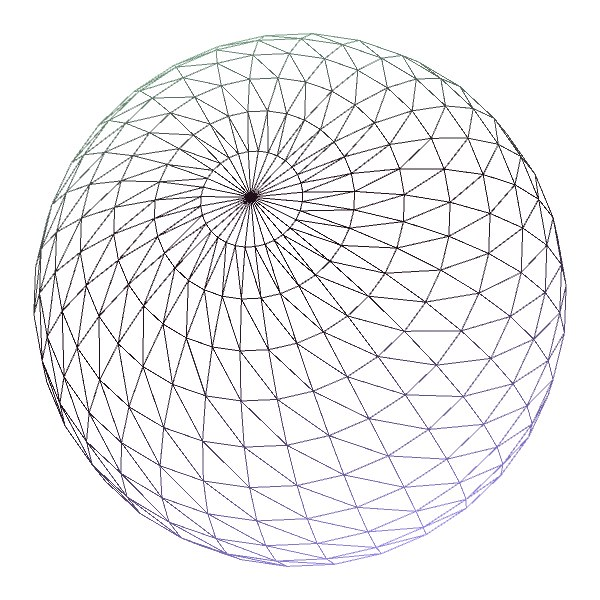
\includegraphics[height=0.8\textheight]{sphere}
	\end{center}
\end{frame}



\end{document}
